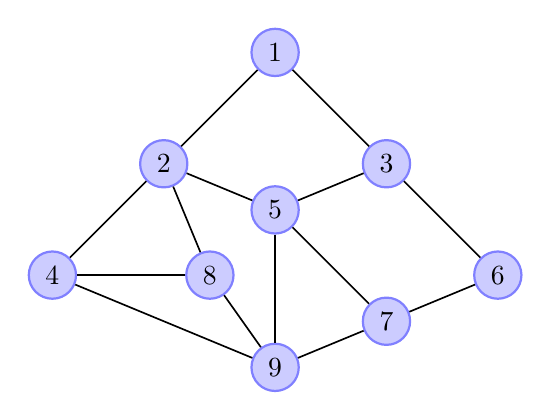
\begin{tikzpicture}[node distance=2cm,semithick,inner sep=1pt,bend angle=45,auto]
%\draw[help lines] (-3,-3) grid (3,0);
\tikzstyle{state}=[circle,draw=blue!50,fill=blue!20,thick,inner sep=0pt,minimum size=6mm]
\node[state]   (v1)                     {1};
\node[state]   (v2) [below left  of=v1] {2};
\node[state]   (v3) [below right of=v1] {3};
\node[state]   (v4) [below left  of=v2] {4};
\node[state]   (v5) [below       of=v1] {5};
\node[state]   (v6) [below right of=v3] {6};
\node[state]   (v7) [below right of=v5] {7};
\node[state]   (v8) [right       of=v4] {8};
\node[state]   (v9) [below       of=v5] {9};

\path
(v1) edge node{} (v2)
     edge node{} (v3)
(v2) edge node{} (v4)
     edge node{} (v5)
     edge node{} (v8)
(v3) edge node{} (v5)
     edge node{} (v6)
(v4) edge node{} (v8)
     edge node{} (v9)
(v5) edge node{} (v7)
     edge node{} (v9)
(v6) edge node{} (v7)
(v7) edge node{} (v9)
(v8) edge node{} (v9);                     
\end{tikzpicture}